\documentclass{article}
\usepackage[utf8]{inputenc}

\title{ENM155 Modellering av hållbara energisystem\\Tentakit}
\author{Jesper Ivarsson}
\date{November 2016}

\usepackage{mathtools}
\usepackage{graphicx}
\usepackage{url}
\usepackage{siunitx}

\begin{document}

\maketitle

\section{Introduktion}
Detta är ett tentakit för kursen ENM155 Modellering av hållbara energisystem. Kursen ges för studenter i årskurs 3 på D-programmet på Chalmers Tekniska Högskola. Kursen tillhör Institutionen för Energi och miljö, avd. Fysisk resursteori. Examinatorer är Frances Sprei och Fredrik Hedenus. \\
\\
Kursen är speciell då tentan enbart är på 3 hp och ges i läsvecka 5. Därav borde tentan vara relativt lätt, då den bara ska examinera de fyra första veckorna. Jag säger borde, då jag i skrivande stund pluggar för att skriva tentan för femte gången.
\\
Dokumentet är uppdelat i olika sektioner. Först presenteras några definitioner, sedan ett gäng tentafrågor, varav en del med svar. Alla svar som presenteras är antingen från exempeltentor från PingPong eller från examinatorernas slides. Därav borde svaren vara någorlunda vettiga att ge på en tenta.

\section{Definitioner och teori}
\subsection{Hållbar utveckling}

1987 presenterades konceptet "Hållbar utveckling". Det lanserades i rapporten "Our common future"\footnote{\url{https://en.wikipedia.org/wiki/Our_Common_Future}}, senare även känd som Brundtland-rapporten. Detta för att kommissionen leddes av den dåvarande norska statsministern Gro Harlem Brundtland.

Den vanligaste definitionen av hållbar utveckling lyder: "Hållbar utveckling är utveckling som tillgodoser dagens behov utan att riskera kommande generationers möjlighet att tillgodose sina behov". Denna definition är värd att lägga på minnet då den ofta efterfrågas på tentan. Den är även det bästa sättet att förklara vad hållbar utveckling faktiskt innebär. 

\subsubsection{De tre dimensionerna}
Det finns tre dimensioner av Hållbar utveckling. Det är vanligt att hela eller delar av dessa defintioner efterfrågas på tentan, därför kör vi igenom dem här! Ibland efterfrågas även "Två viktiga komponenter" inom varje dimension, vi går igenom några sådana med.\\
\\
\textbf{Den ekologiska dimensionen}\\
\ \\
Den ekologiska dimensionen innebär att man även i framtiden ska ha naturliga system som kan försörja människor. Exempel på detta är produktiv jordbruksmark, naturlig vattenrening och att begränsa utsläp av kemikalier till den nivå naturen klarar av att hantera.\\
\\
\textbf{Den ekonomiska dimensionen}\\
\ \\
Den ekonomiska dimensionen innebär att hushålla med resurser som är viktiga för mänsklig välfärd. Det handlar både om naturkapital, som exempelvis fossila bränslen, men också om resurser som människor skapat, exempelvis infrastruktur, byggnader och fabriker.\\
\\
\textbf{Den sociala dimensionen}\\
\ \\
Den sociala dimensionen innebär att bygga och bevara sociala institutioner som främjar välbefinnande, exempelvis fungerande rättsstat, tillit mellan människor, demokrati samt mänskliga rättigheter.

\subsection{Växthuseffekt}
Växthuseffekten är du förmodligen redan bekant med. Men vet du exakt hur den fungerar? Inte? Lugn, miljökursen got your back. På tentan brukar man bli ombedd att förklara vad växthuseffekten är och hur den fungerar rent fysikaliskt. Lite random fakta kommer även efterfrågas.\\
\\
\textbf{Fysiken bakom naturlig växthuseffekt}\\
\\
Jorden måste avge lika mycket värmestrålning som den tar emot, annars skulle temperaturen stiga. En bra glosa här är \textit{albedo}. Albedo är ett mått som anger hur stor del av solstrålningen som vid marken eller molnen studsar tillbaka ut i rymden. Albedo anges som en faktor mellan 0 och 1, där 0 är inget och 1 är allt. \textbf{EJ FÄRDIGSTÄLLD}\\
\\
\textbf{De viktigaste \textit{naturliga} växthusgaserna}\\
\\
De viktigaste naturliga växthusgaserna är, i fallande ordning:
\begin{itemize}
    \item Vatten
    \item Koldioxid
    \item Ozon
\end{itemize}
Svårare än så är det inte!\\
\\
\textbf{De viktigaste \textit{antropogena} växthusgaserna}\\
\\
En antropogen växthusgas är en gas som människan har bidragit till att skapa\footnote{\url{https://sv.wikipedia.org/wiki/Antropogen}}. Det är alltså gaser som släpps ut av transporter, industrier, boskap m.m. De viktigaste av dessa gaser är:
\begin{itemize}
    \item{Koldioxid ($CO_2$)}
    \begin{itemize}
        \item[--] Kommer huvudsakligen ur fossila bränslen men även genom avskogning, då träd absorberar koldioxid.
    \end{itemize}
    \item{Metan ($CH_4$)}
    \begin{itemize}
        \item[--] Nötdjur
        \item[--] Jordbruk
        \item[--] Avfall
        \item[--] Utvinning av fossia bränslen
    \end{itemize} 
    \item{Lustgas ($N_2O$)}
    \begin{itemize}
        \item[--] Konstgödsel för jordbruk
    \end{itemize}
    \item{Flourerade gaser ($HCF$, $PFC$, $SF_6$)}
    \begin{itemize}
        \item[--] Kylmedel och i elektronik
    \end{itemize}
\end{itemize}

\subsection{Resurser och reserver}

Du kommer nästan garanterat att få frågan om resurser, reserver och dynamiken mellan dem, så det är lika bra att du lär dig detta nu. Resurser är den totala förekomsten av ett ämne på jorden. Olja är ett bra exempel på detta. Reserver är ett namn för den delmängd av resurserna som är känd och kan utvinnas till ett marknadsmässigt pris. En oljeficka kan därmed vara känd, men vara såpass svåråtkomlig att den klassas som resurs. Om reserverna sinar så stiger priset. Det får två effekter:
\begin{itemize}
    \item Man börjar att leta efter nya fyndigheter.
    \item Man börjar utvinna resurser som tidigare varit för dyra att utvinna. Detta leder till att reserverna utökas.
\end{itemize}
För att få full pott på denna fråga, eller snarare för att gardera dig mot poängavdrag, bör du rita upp figur \ref{fig:reservresurs}. Det har hänt förr att examinatorerna dragit av både en och två poäng för att figuren saknats.
\begin{figure}[!ht]
    \centering
    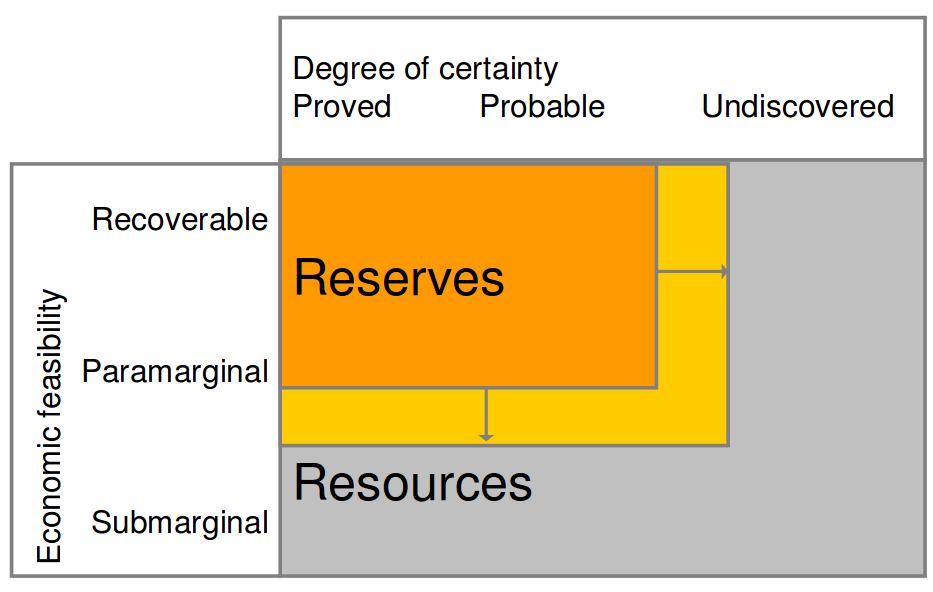
\includegraphics[width=50mm]{resurs.png}
    \caption{Dynamiken mellan resurser och reserver}
    \label{fig:reservresurs}
\end{figure}

\subsection{Load factor}
Load factor är en tuff grej som du verkligen vill ha koll på! Detta är en av två räkneuppgifter som då och då dyker upp på tentorna. Load factor betecknar hur stor del av tiden som något jobbar på full effekt, se ekvation nedan.\\
\begin{equation}
Load~factor = \frac{Faktisk~produktion}{Högsta~möjliga~produktion}
\end{equation}


På tentorna används ofta vindkraftverk som exempel. Därför tänker jag ta det som exempel med.\\
\\
\textit{Ett vindkraftverk har en effekt på 3 MW. På ett år genererar det 10,5 GWh. Hur hög är load factor?}
\begin{equation}
\begin{aligned}
    P_{vindkraft} = \SI{3}{\mega\watt}\\
    P_{år} = \SI{10500}{\mega\watt\hour}\\
    P_{max} = 365 \times 24 \times \SI{3}{\mega\watt\hour} = \SI{26280}{\mega\watt\hour}\\
    Load~factor = \frac{P_{år}}{P_{max}} = \frac{10500}{26280} = 0.3995... = 0.4\\
\end{aligned}
\end{equation}

\subsubsection{Övriga frågor kring load factor}
\textit{Vad menas med ett kraftverks loadfactor?}\\
\\
Load factor är ett mått på hur stor andel av året som ett kraftverk levererar el vid full effekt.\\
\\
\textit{Ge tre exempel på anledningar som gör att ett kraftverks loadfactor är lägre än 100 procent}
\begin{itemize}
    \item Vindkraftverk levererar inte när det vindstilla och solceller levererar inte när det är natt.
    \item Man kan behöva stanna vindkraftverk för att göra underhåll
    \item Elpriset kan under perioder vara för lågt för att vindkraftverket ska vara lönsamt att driva.
\end{itemize}

\subsection{Verkningsgrad och koldioxidutsläpp}
Alla som klarat Fysik A borde redan ha koll på detta. Du borde dessutom ha läst Fysik för ingenjörer vid det här laget, så det är ännu orimligare att jag ska förklara det för dig. Men visst.\\
\\
Verkningsgrad är ett mått på effektivitet. Den betecknas med den grekiska bokstaven \si{\eta} (eta) och definieras som:
\begin{equation}
\si{\eta} = \frac{P_{ut}}{P_{in}}
\end{equation}
Denna formel vävs på tentorna ofta in i en uppgift där man beräknar koldioxidutsläpp. Vi tar och kör en sån uppgift direkt och får kläm på det!\\
\\
\textit{Stenkol orsakar utsläpp på \SI{90}{\gram~CO_2\per\mega\joule}. Stenkol har vid förbränning en verkningsgrad på \SI{35}{\percent}. Beräkna utsläppen koldioxid per \si{\kilo\watt\hour}}\\
\\
\begin{equation}
\begin{aligned}
\SI{1}{\joule} = \SI{1}{\watt\second}\\
\SI{3600}{\joule} = \SI{1}{\watt\hour}\\
\SI{3,6}{\mega\joule} = \SI{1}{\kilo\watt\hour}\\
\end{aligned}
\end{equation}
\begin{equation}
\begin{aligned}
CO_2~per~\si{\kilo\watt\hour} = \frac{\si{\gram}~CO_2/\si{\mega\joule} \times 3,6}{\si{\eta}} = \frac{90 \times 3,6}{\si{0,35}} = 925,714... = 926
\end{aligned}
\end{equation}

\subsection{Koldioxidutsläpp inom transportsektorn}

Det är givetvis högaktuellt att diskutera koldioxidutsläppen inom transportsektorn. Det är det alltid och det är ett återkommande tema på denna kurs tentor. Man brukar bli tillfrågad om tre principiellt olika strategier för att minska utsläppen inom transportsektorn. Så vilka är då dessa tre?\\
\\
\textbf{Minskad efterfrågan}\\
\\
Minskad efterfrågan nås genom minskad användning. Samåkning, kollektivtrafik och elbilar är några exempel på hur man kan minska användningen.. Andra medel är ökad cykeltrafik och trängselskatter.
\\
\\
\textbf{Byte av bränsle}\\
\\
Bränslen kan bytas ut mot sådana med mindre miljöpåverkan, exempelvis elbilar som går på grön el. Även biodiesel och biogas som (åtminstone i teorin) är klimatneutrala.\\

\newpage
\\
\textbf{Energieffektiviseringar}\\
\\
Man kan sist men inte minst effektivisera användningen. Motorer kan optimeras, rull- och luftmotstånd minskas och man kan använda appar för att effektivisera rutter och transporter för att resa kortast möjliga väg.
\subsection{Koldioxidskatter}
Koldioxidskatter är ett incitament för att bidra till minskade koldioxidutsläpp. Detta får tre prinicipiellt olika effekter på ett energisystem.
\begin{itemize}
    \item \textbf{Effektivisering} 
    \begin{itemize}
        \item[--] Bättre isolering
        \item[--] Effektiva metoder
    \end{itemize}
    \item \textbf{Teknikbyte}
    \begin{itemize}
        \item[--] Byte från mer till mindre koldioxidintensiva tekniker
    \end{itemize}
    \item \textbf{Miskad efterfrågan}
    \begin{itemize}
        \item[--] Minskad körning
        \item[--] Svalare inomhustemperatur
    \end{itemize}
\end{itemize}

\subsection{Andra koldioxidbestraffningar}
Det finns två huvudsakliga sätt att prissätta koldioxid. Beskattning och utsläppshandel.

Beskattning gör att utsläppen får ett fast och förutsägbart pris men det är oklart hur stor minskningen av utsläpp blir.

Utsläppshandel för att man istället får en förutsägbar maximal mängd utsläpp.

\subsection{Annat om koldioxid}

Om mängden $CO_2$ i atmosfären fördubblas så stiger medeltemperaturen med 1.1 grader.\\
\\
För att nå tvågradersmålet måste utsläppen av $CO_2$ upphöra helt om klimatkänsligheten är hög, är den låg kan vi fortsätta lite till. Eventuellt kommer ett tregradersmål bli aktuellt istället.


\subsection{Hantering av variabel elproduktion}

Det finns tre övergripande strategier för att hantera stora mängder variabel elproduktion. Men först, vad är variabel elproduktion egentligen? Motsatsen, som vi kan kalla statisk (oklart om detta är ett korrekt namn) elproduktion, är den produktion man kan reglera. Man kan reglera styrstavarna i ett kärnkraftverk och man kan reglera vattnet till turbinerna i Norrlands älvar. Vad man däremot inte kan rå på är väder och vind. Därför sägs sol- och vindelsproduktion vara variabel. Energikällan är därför opålitlig och måste optimeras för att vara hållbar. Men vilka är dessa strategier för att hantera elproduktionen?\\
\\
\textbf{Transmissionsnät}\\
\\
Ett utbyggt transmissionsnät gör att man kan skicka el dit den behövs. På sommaren, när sydeuropa kräver mycket el till kylaggregat kan ström tas från nordeuropa. På samma sätt kan el förflyttas på vintern när norra Europa behöver el till uppvärmning. Genom att ha vindkraft på olika platser produceras el vid olika tillfällen, vilket ger en jämn elförsörjning.\\
\\
\textbf{Lagring}\\
\\
Man kan använda lagringstekniker för att spara el från dagar med god elförsörjning till dagar med sämre elförsörjning. Exempelvis från en blåsig och solig dag till en vindstilla natt.\\
\\
\textbf{Justering av efterfrågan}\\
\\
Man kan justera efterfrågan genom att inte förbruka så mycket el när tillgången är låg. Ett bra exempel är att bara tvätta på dagen när det är sol, och inte på natten när det kanske är vindstilla.\\
\\
\textbf{Geografisk spridning}\\
\\
Genom att sprida ut kraftverken geografiskt blir chansen större att det blåser på någon av platserna, och på så sätt stabiliserar tillgången på vinkraftsel. Detsamma gäller för solkraft.

\subsection{Kärnkraft}

Kärnkraft sägs ju vara en bra grej, allt som oftast. Men vad man ofta inte tänker på är att de tekniker som används för kärnkraftverk även kan användas för att framställa kärnvapen. Det är nämligen så att man med samma teknik som används för att anrika Uran-235 till 4-5 procent för  kärnkraft, kan anrika Uran-235 till 90 procent, vilket kan användas i kärnvapen.\\
\\
Utbränt kärnbränsle kan upparbetas, vilket innebär att Plutonium separeras, för att sedan användas som bränsle. Plutonium från reaktorer kan potentiellt användas för att göra kärnvapen. Här finns dock vissa tekniska utmaningar.\\
\\
Tyvärr kan civila anläggningar för hantering av radioaktiva material användas som täckmantel för militära ändamål.\\
\\
Dessutom kan kunskapen om kärnklyvning och materialhantering som sprids i ett civilt kärnkraftsprogram också användas för att tillverka kärnvapen.

\subsection{Bioenergins koldioxidneutralitet}

Bioenergi som förbränns orsakar utsläpp av cirka \SI{110}{\g $CO_2$/\mega\joule}, så hur kommer det sig att man ändå betraktar bioenergi som koldioxidneutralt? Jo, för att utsläppen av $CO_2$ som förbränningen av bioenergin orsakar motsvarar precis den mängd $CO_2$ som plantan absorberar från atmosfären under sin uppväxt. För att bioenergin ska vara koldioxidneutral så måste det planteras nya grödor i samma omfattning efter skörd.


\section{Tentauppgifter}

I detta avsnitt finns rena tentafrågor med svar att plugga på.

\subsection{Klimatkänslighet}
\textit{Klimatkänslighet är ett centralt begrepp inom klimatvetenskapen. Definiera begreppet och förklara kortfattat varför det är så centralt för diskussionen om hur tvågradersmålet ska nås.}\\
\\
Klimatkänsligheten är ett mått på hur starkt växthusgaser påverkar jordens temperatur. Oftast anges känsligheten som den globala medelökningen i lufttemperatur vid jordytan om man fördubblar atmosfärens $CO_2$-koncentration jämfört med förindustriell nivå. Det finns många olika uppskattningar av känsligheten i ett ganska stort intervall. Debatten om känsligheten är mycket svår och viktig eftersom vårt kvarvarande utsläppsutrymme för tvågradersmålet skiljer sig mycket kraftigt även om man bara varierar känsligheten inom det intervall som IPPC anser är mest troligt.

\subsection{Fyra faktorer i energisystemet}

\textit{Nämn de fyra faktorer som påverkar energisystemet enligt Johansson (2013) och ge ett centralt exempel för varje faktor, samt motivera varför det kommer påverka utvecklingen av det svenska energisystemet.}

\begin{itemize}
    \item \textbf{Teknik}
    \begin{itemize}
        \item[--] Beroende på hur priset för vindkraft globalt utvecklas så kommer det få betydelse för hur vindkraften sprids i Sverige, eftersom det påverkar konkurrenssituationen med andra tekniker såsom kärnkraft och naturgas.
    \end{itemize}
    \newpage
    \item \textbf{Politik}
    \begin{itemize}
        \item[--] Om man politiskt bestämmer sig för att avveckla kärnkraften har det betydelse för kraftförsörjningen. Om man ökar eller minskar koldioxidskatten påverkas konkurrenskraften för t.ex. biobränsle.
    \end{itemize}
    \item \textbf{Ekonomi}
    \begin{itemize}
        \item[--] Den ekonomiska tillväxten i Sverige kommer ha betydelse för efterfrågan på energi, eftersom tillväxt och energianvändning historiskt varit nära kopplade.
    \end{itemize}
    \item \textbf{Naturresurser}
    \begin{itemize}
        \item[--] Om oljan sinar globalt och priset skjuter i höjden så kommer det få betydelse för introduktionen av elbilar, då det gör dem mer konkurrenskraftiga mot bensin- och dieselbilar.
    \end{itemize}
\end{itemize}

\subsection{Skillnader i transportsektorn}
\textit{Transportsektorn skiljer sig från andra sektorer (såsom jordbruk, bostäder och industri) när det gäller trender inom energianvändning och utsläpp. Förklara kortfattat skillnaden.}\\
\\
Transportsektorns utsläpp har fortsatt att öka och deras andel av utsläppen ökar ju rikare ett land blir, till skillnad från de andra sektorerna. Transportsektorn upptar också en större andel av oljeanvändningen och har inte i samma utsträckning lyckats substituera olja med andra bränslen.

\subsection{Energieffektiviseringar}

\textit{I föreläsningen om energieffektiviseringar presenterades olika potentialer för att minska energianvändingen genom energieffektivisering. Nämn tre av dessa potentialer och förklara vilka faktorer som avgör hur stor eller liten potentialen är.}

\begin{itemize}
    \item Teoretisk potential
    \begin{itemize}
        \item[--] Beror på grundläggande naturlagar om bevarande av massa och energi.
    \end{itemize}
    \item Teknisk potential
    \begin{itemize}
        \item[--] Kommer att variera mellan sektorer och beror på bästa tillgängliga teknik.
        \item[--] Närmar sig över tid den teoretiska potentialen.
    \end{itemize}
    \item Ekonomisk potential
    \begin{itemize}
        \item[--] Beror på energipriser och räntor.
    \end{itemize}
    \item Marknadspotential
    \begin{itemize}
        \item[--] Liknar den ekonomiska potentialen men kommer bero på aktuella räntor och avskrivningskalkyler hos olika marknadsaktörer.
    \end{itemize}
\end{itemize}

\subsection{Havsnivåhöjning}

\textit{Det finns två huvudsakliga anledningar till att havsnivån höjs vid ett varmare klimat. Vilka är dessa?}\\
\\
Först och främst leder högre temperatur till att glaciärer, arktis och antarktis smälter. Men högre temperatur bidrar även till termisk expansion, det vill säga att vattnet expanderar vid högre temperatur.

\subsection{Energieffektiviseringar}

\textit{Beskriv tre olika övergripande förklaringar/drivkrafter till att energieffektiviseringar ökar inom en sektor eller industri}
\begin{itemize}
    \item Vanlig omsättning av teknik
    \item Förbättring av drift
    \item Ekonomiska besparingar
    \item Politiskt tryck
    \end{itemize}
    
\subsection{Kärnkraftsreaktorer}

\textit{Ange de två viktigaste energigivande reaktionerna för frigörande av energi i en lätt vattenreaktor.}
\begin{equation}
\begin{aligned}
    $U_{235}$ + $1_n$ \rightarrow X + Y + $2-3_n$ + E \\
    $U_{238}$ + $1_n$ \rightarrow $Pu_{239}$ \\
    $Pu_{239}$ + $1_n$ \rightarrow X + Y + $2-3_n$ + E\\
\end{aligned}
\end{equation}

\subsection{Begränsningar i bioenergi}

\textit{Tillgången till bördig mark är den största begränsningen för hur mycket bioenergi som kan användas i världen. Beskriv två olika åtgärder för att frigöra mark så att mer bioenergi kan produceras i framtiden.}\\
\\
\begin{itemize}
    \item Övergivna odlingsmarker
    \item Betesmarker
    \item Yield gap
    \item Integrerade produktionssystem
\end{itemize}

\subsection{Framtidsscenarier}

\textit{Man kan beskriva framtidsscenarier som antingen deskriptiva, explorativa eller normativa. Beskriv kortfattat vad dessa olika typer av scenarier innebär, och ge energirelaterade exempel på när vart och ett av dem är rimligt att använda.}
\begin{itemize}
    \item Deskriptiv
    \begin{itemize}
        \item[--] Beskrivande
    \end{itemize}
    \item Normativ
    \begin{itemize}
        \item[--] Vägledande
    \end{itemize}
    \item Explorativ
    \begin{itemize}
        \item[--] Undersökande
    \end{itemize}
\end{itemize}

\end{document}
